\documentclass[aspectratio=169,cramped]{beamer}
\usetheme[minimal,infbio]{tugraz2018}
\usepackage[utf8]{inputenc}
\usepackage{booktabs}
\usepackage{varwidth,lipsum}
\newcommand\hide[1]{\phantom{\varwidth{\linewidth}#1\endvarwidth}}
\usepackage{ulem}
\usepackage[ttscaled=0.8,tt=false]{libertine}

\usepackage{tikz}
\usepackage{tikz-qtree}

\hypersetup{colorlinks,urlcolor=blue,linkcolor=}
\let\tempone\itemize
\let\temptwo\enditemize
\renewenvironment{itemize}{\tempone\addtolength{\itemsep}{-0\baselineskip}\addtolength{\parskip}{-0.2\baselineskip}}{\temptwo}
\newcommand{\putat}[3]{\begin{picture}(0,0)(0,0)\put(#1,#2){#3}\end{picture}}
\newcommand{\ex}[1]{{\color{teal} #1}}
\newcommand{\checkyes}{\textcolor{tuggreen}{\faCheckSquareO}}
\newcommand{\checkno}{\textcolor{black}{\faSquareO\,}}
\newcommand{\bulletplus}{\textcolor{tuggreen}{\faPlusCircle}}
\newcommand{\bulletminus}{\textcolor{tugred}{\faMinusCircle}}
\newcommand{\bulletconclusion}{\textcolor{tugblue}{\faArrowCircleRight}}

\title{Natural Language Processing: \\ How do humans process language?}
% \subtitle{Natural Language Processing}
\author{Philipp Gabler <pgabler@student.tugraz.at>}
\instituteurl{}
\date{2020-05-07}

\begin{document}

\begin{frame}
    \titlepage
\end{frame}

\begin{frame}{Outline}
    \tableofcontents
\end{frame}


%//////////////////////////////////////////////////////////////////////
\sectionheader[What does NLP have to do with humans, at all?]{\textbf{Motivation}}
\section{Motivation}

\begin{frame}{Linguistics \& NLP}
  \textbf{Too much theory is bad? But why?}
	\begin{itemize}
  \item ``Every time I fire a linguist, the performance of the speech processing system goes up.''
    (Frederick Jelinek)
  \item Does it mean we should refrain from linguistic inspiration?
    \begin{itemize}
    \item (NLP already does that.  Ask a linguist.)
    \end{itemize}
  \item Cf. the good, bad, and ugly parts of artificial neural networks
	\end{itemize}
\end{frame}

\begin{frame}{Levels of Abstraction}
	\textbf{Linguists and Engineers tend to have different focus}
	\begin{itemize}
  \item Computational: what is explained?
    \begin{itemize}
    \item \ex{Description of linguistic performance vs. explanation of linguistic competence}
    \end{itemize}
  \item Algorithmic: how is it done?
    \begin{itemize}
    \item  \ex{Cognitive realism, computational complexity/efficiency}
    \end{itemize}
  \item Implementational: how is is realized?
    \begin{itemize}
    \item  \ex{Neurological plausibility}
    \end{itemize}
  \end{itemize}
\end{frame}

\begin{frame}{Insights \textit{from} linguistics}
	\textbf{Get a better understanding of what should work in language processing}
	\begin{itemize}
  \item After all, it's \emph{natural language} processing
  \item Comparison gives confidence:
    \begin{itemize}
    \item NLU system behaviour vs. L1 acquisition
    \item Observation of similar effects/errors, e.g., garden path sentences
    \item Human performance is the ultimate (utopic?) benchmark!
    \item We're not inventing something \emph{new}\ldots
    \end{itemize}
  \end{itemize}
\end{frame}

\begin{frame}{Insights \textit{for} linguistics}
	\textbf{We don't yet know how human language really works}
	\begin{itemize}
  \item Very conflicting hypotheses, most of which work only on a computational level
  \item New ideas:
    \begin{itemize}
    \item Shallow processing
    \item Distributed, implicit, usage-based knowledge
    \item Computational construction grammar
    \item Computational semantics (\(\lambda\) calculus)
    \end{itemize}
  \end{itemize}
\end{frame}

\begin{frame}{Some words of caution}
  \textbf{Be warned!}
  \begin{itemize}
  \item This is will be an extremely rough, simplified, and incomplete overview
  \item It is biased in favour of Cognitive Linguistics (and a bit against Generative Grammar)
  \item Linguistic theory is not completely scientific
    \begin{itemize}
    \item ``Theory'' = ``proposed descriptive model'', not ``axiomatic system''
    \end{itemize}
  \item If you're interested: go to the linguistics department
    \begin{itemize}
    \item
      \href{https://online.uni-graz.at/kfu_online/wbLv.wbShowLVDetail?pStpSpNr=584778}{Sprache und Kognition}, \href{https://online.uni-graz.at/kfu_online/wbLv.wbShowLVDetail?pStpSpNr=582944&pSpracheNr=1}{Sprachen
      der Welt}, \ldots
    \item Learn more languages (for grammar, not talking)
    \end{itemize}
  \end{itemize}
\end{frame}

%//////////////////////////////////////////////////////////////////////
\sectionheader[Some examples from different areas of linguistics and cognitive science]{\textbf{Models of human language}}
\section{Models of human language}

\begin{frame}{Cognitive \& Linguistic Development}
	\textbf{Cognitive abilities develop in similar ways}
	\begin{itemize}
  \item Typical progress:
    \begin{itemize}
    \item Statistical learning (expectation \& surprise)
    \item Inductive learning (categorization \& abstraction)
    \item Social learning (imitation, intention, theory of mind)
    \end{itemize}
  \item Sensomotory system has an important influence in learning!
  \item Critical periods vs. extreme robustness
  \end{itemize}
\end{frame}

\begin{frame}{Language acquisition}
	\textbf{Language learning tends to follow a U-shaped progress}
	\begin{itemize}
    \item Phases:
    \begin{itemize}
    \item Simplification: \ex{How do you do dese\ldots work/tortillas/in English}
    \item Overgeneralization: \ex{Yesterday I didn’t painting}
    \item Restructuring \ex{How do you\ldots make this/like it; how\ldots do cut it}
    \end{itemize}
  \item Cf. exploration vs. exploitation in reinforcement learning
  \item Computational and associative learning
  \end{itemize}
\end{frame}

\begin{frame}{Creolization processes}
  \vspace{-1cm}
  \begin{figure}
    \centering
    \includegraphics[width=7cm]{figures/hotel-sign.jpg}
    \caption{Hotel room signs in Tok Pisin (Papua New Guinea)}
  \end{figure}
  \vspace{-.1cm} \tiny \url{https://en.wikipedia.org/wiki/Subject\%E2\%80\%93object\%E2\%80\%93verb}
\end{frame}

\begin{frame}{Universal Grammar}
	\textbf{Generative Grammar = trees + transformations}
	\begin{itemize}
  \item Grammatical construal in terms of rules
    \begin{itemize}
    \item from \emph{deep structure} to \emph{surface structure}
    \end{itemize}
  \item Exlaining all languages in terms of \emph{principles and parameters}
    \begin{itemize}
    \item Solution to fast, one-shot L1 acquisition
    \end{itemize}
  \end{itemize}
\end{frame}

\begin{frame}{Triangles in the brain?}
  \begin{figure}
    \centering
    \vspace{-2cm}
    \hspace{1cm}
    \begin{tikzpicture}
      % \tikzset{frontier/.style={distance from root = 5cm}}
      \tikzset{level distance=8mm}
      \Tree [.CP [.\={C} C [.IP [.NP [.Det The ] [.\={N} [.N children ] ] ]
            [.\={I} [.I should ] [.VP [.\={V} [.V have ] [.VP [.\={V} [.V waited ] ] ] ] ] ] ] ] ]
    \end{tikzpicture}
  \end{figure}
\end{frame}

\begin{frame}{Triangles in the brain?}
  \begin{figure}
    \centering
    \vspace{-2cm}
    \hspace{1cm}
    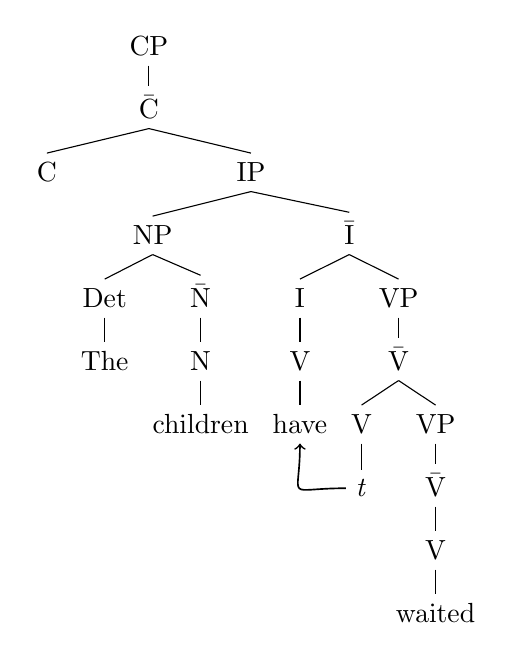
\begin{tikzpicture}
      \tikzset{level distance=8mm}
      \Tree [.CP [.\={C} C [.IP [.NP [.Det The ] [.\={N} [.N children ] ] ]
            [.\={I} [.I [.V \node(i){have}; ] ] [.VP [.\={V} [.V \node(t){\textit{t}}; ] [.VP [.\={V} [.V waited ] ] ] ] ] ] ] ] ]
      \draw[semithick,->] (t).. controls +(west:1) and +(south:1)..(i);
    \end{tikzpicture}
  \end{figure}
\end{frame}

\begin{frame}{Universal Grammar}
	\textbf{Criticism of this kind of analysis}
  \begin{itemize}
  \item Explicitely not empirical (at least by Chomsky)
    \begin{itemize}
    \item Against ``behaviourism'', focus on competence
    \item Tends to categorize everything in terms of recursive symbolic structures
    \item Good for English~-- what about Chinese? Pirah\~{a}?
    \end{itemize}
  \item Computationally complex, cognitively\ldots difficult to explain
  \end{itemize}
\end{frame}

\begin{frame}{Representations of meaning}
	\textbf{Language is conveying mental state through symbols}
  \begin{itemize}
  \item Semantics from a cognitive perspective: meaning is\ldots
    \begin{itemize}
    \item perspectivic (relative to utterance context)
    \item dynamic (system changes with environment)
    \item encyclopedic (association with experiences \& culture)
    \item determined by usage (a system derived from concrete experience)
    \end{itemize}
  \item Grammar is only an ``artifact'' to structure the transportation of mental state
    \begin{itemize}
    \item Or: only an instrument for performative utterance
    \end{itemize}

  \end{itemize}
\end{frame}


% \begin{frame}{Influential Early Work}
%     \textbf{Syntactic Structures by Noam Chomsky} (1957)
%     \begin{itemize}
%         \item Book (lecture notes) proposing to analyse the structure of text
%         \begin{itemize} 
% 			\item ... and transforming it, so that machine can process them
% 			\begin{itemize}
% 				\item Phase-Structure Grammar
% 			\end{itemize}
%         \end{itemize}
% 		\item ``\textit{Colorless green ideas sleep furiously}''
% 		\begin{itemize}
% 			\item \textbf{Grammatically} correct, but \textbf{semantically} meaningless
% 			\item Plus, an example for a sentence that has never been formulated before
% 		\end{itemize}
%     \end{itemize}
% \end{frame}
% \begin{frame}{Influential Early Work}
%     % \textbf{Syntactic Structures by Noam Chomsky} (1957)
%     \begin{itemize}
%         \item ``Early claims that computers can translate languages were vastly exaggerated''
%         \begin{itemize} 
% 			\item Anthony Oettinger (1966)
%         \end{itemize}
% 		\item ``\textit{Time flies like an arrow}'' as example for an ambiguous sentence
% 		\begin{itemize}
% 			\item ... time moves quickly? (figuratively)
% 			\item ... measure the speed of flies? (imperative)
% 			\item ... species ``time flies'' have a preference for arrows?
% 		\end{itemize}
%     \end{itemize}
% \end{frame}
% \begin{frame}{ELIZA}
%     \centering
% 	\includegraphics[width=8cm]{images-history/ELIZA_conversation.jpg} \\
%     \small Developed by Joseph Weizenbaum at MIT (1964-66) 
% \end{frame}
% \begin{frame}{First AI Winter}
%     \textbf{Little progress} 
%     \begin{itemize}
%         \item NLP (and other AI-related topics) received less funding
%         \item ... due to failure to deliver, e.g., a working machine translation systems
%         \item $\rightarrow$ relatively little (visible) progress achieved
%         \begin{itemize}
% 			\item during the late 60ties to early 80ties
%         \end{itemize}
%     \end{itemize}
% \end{frame}
% \begin{frame}{Knowledge Representation}
%     \textbf{History of knowledge representation} 
%     \begin{itemize}
%         \item Field of AI, closely related to NLP 
% 		\item General Problem Solver (1959)
% 		\begin{itemize}
% 			\item Computer program 
% 			\begin{itemize}
% 				\item Could solve ``toy examples''
% 				\item Dedicated programming language
% 			\end{itemize}
% 			\item Separated knowledge from the solving itself
% 		\end{itemize}
% 		\item Expert systems
% 		\begin{itemize}
% 			\item Introduced by Feigenbaum (1965)
% 			\item Knowledge-based and reasoning system
% 		\end{itemize}
%     \end{itemize}
% \end{frame}
% \begin{frame}{Knowledge Representation}
% 	\putat{290}{-180}{\includegraphics[height=1.1\textheight]{images-history/kicktionary.png}}
%     \textbf{Types of knowledge representation} 
%     \begin{itemize}
% 		\item Frame
% 		\begin{itemize}
% 			\item Inspired by psychological research (1930ties)
% 			\item Structures knowledge in hierarchical relationships
% 			\begin{itemize}
% 				\item e.g., KL-ONE (1977), FrameNet (1997)
% 				\item Kicktionary: \url{http://www.kicktionary.de}
% 			\end{itemize}
% 		\end{itemize}
% 		\item Semantic networks
% 		\begin{itemize}
% 			\item Inspired by associational memory of humans
% 			\begin{itemize}
% 			 \item e.g., Aschaffenburg (early 20th century)
% 			\end{itemize}
% 			\item Cyc (1984)
% 			\item Ontologies, e.g., RDF \& OWL
% 		\end{itemize}
%     \end{itemize}
% \end{frame}
% \begin{frame}{Semantic Net}
%     \centering
% 	\includegraphics[width=8cm]{images-history/1920px-Semantisches_netz.png} \\
%     \small Example of an early semantic net (Collins und Quillian, about 1960s) 
% \end{frame}
% \begin{frame}{Ontologies}
% 	\begin{itemize}
% 		\item In philosophy an ontology deals with the existence question
% 		\item Since 1980s the term is being using in computer science
% 		\item Main components
% 		\begin{itemize}
% 			\item Individuals (instances), classes (concepts), attributes and relations
% 			\item Whereas relations often can be freely defined
% 		\end{itemize}
% 		\item Upper ontologies vs. domain ontologies
% 		\begin{itemize}
% 			\item Only a few upper ontologies
% 		\end{itemize}
% 	\end{itemize}
% \end{frame}
% \begin{frame}{Knowledge Graph}
% 	\textbf{Ontologies are still popular today}
% 	\begin{itemize}
% 		\item Term coined by Google initiative (2012)
% 		\begin{itemize}
% 			\item Knowledge base represented as a graph
% 		\end{itemize}
% 		\item Well-known example: FreeBase (2007)
% 		\begin{itemize}
% 			\item Graph database (tripe store)
% 			\item Similar projects: YAGO, DBPedia, Wikidata
% 		\end{itemize}
% 		\item Relevant for NLP
% 		\begin{itemize}
% 			\item WordNet
% 			\item ConceptNet
% 		\end{itemize}
% 	\end{itemize}
% \end{frame}
% \begin{frame}{Logic}
% 	\textbf{History of reasoning}
% 	\begin{itemize}
% 		\item Initial combination of rules and logic for inference and reasoning
% 		\begin{itemize}
% 			\item e.g., first-order (predicate) logic
% 		\end{itemize}
% 		\item Notations
% 		\begin{itemize}
% 			\item e.g., context free grammar (BNF)
% 		\end{itemize}
% 		\item Fuzzy logic
% 		\begin{itemize}
% 			\item Introduced by Lotfi A. Zadeh (1965)
% 			\item Following the intuition that decisions do not have ``hard borders''
% 		\end{itemize}
% 	\end{itemize}
% \end{frame}
% \begin{frame}{Corpus Linguistics}
% 	\textbf{History of language corpora}
% 	\begin{itemize}
% 		\item \textit{Brown corpus} (1961)
% 		\begin{itemize}
% 			\item 500 samples of English-language text
% 		\end{itemize}
% 		\item ``Computational Analysis of Present-Day American'' by Henry Kučera and W. Nelson Francis (1967)
% 		\item $\rightarrow$ Frequency of words follow the Zipf's law
% 		\item The Brown corpus was later also tagged
% 		\begin{itemize}
% 			\item Each word was \textbf{annotated} with its word group
% 		\end{itemize}
% 	\end{itemize}
% \end{frame}
% \begin{frame}{Paradigm Shift in NLP}
% 	\begin{itemize}
% 		\item The majority of word in NLP by until the mid 1980s were based on rules
% 		\begin{itemize}
% 			\item e.g., mostly \textbf{hand-crafted rules} 
% 			\item ... using domain knowledge (linguists)
% 		\end{itemize}
% 		\item Shift toward statistical and stochastic models
% 		\begin{itemize}
% 			\item e.g., \textbf{machine learning}
% 			\item ... in combination with corpus linguistics
% 			\item ``\textit{Every time I fire a linguist, the performance of the speech recognizer goes up}''
% 			\begin{itemize}
% 				\item Frederick Jelinek (1985)
% 			\end{itemize}
% 		\end{itemize}
% 		% \item Today: \textbf{Deep Learning}
% 	\end{itemize}
% \end{frame}
% \begin{frame}{Machine Translation as Example for NLP History}
%     \centering
%     \vspace{-1.5cm}
% 	\includegraphics[width=15cm]{images-history/mt-history.png} \\
%     \small \vspace{-1cm} History of machine translation \tiny \url{https://vas3k.com/blog/machine_translation/}
% \end{frame}
% \begin{frame}{Recent History of Deep Learning Based NLP}
% 	\begin{description} \vspace{-.8cm}\setlength\itemsep{0pt}
% 		\item[2001] Neural language models
% 		\item[2008] Multi-task learning
% 		\item[2013] Word embeddings
% 		\item[2013] Neural networks for NLP
% 		\item[2014] Sequence-to-sequence models
% 		\item[2015] Attention
% 		\item[2015] Memory-based networks
% 		\item[2018] Pretrained language models
% 	\end{description}
% 	\scriptsize Taken from: \url{https://ruder.io/a-review-of-the-recent-history-of-nlp/}
% \end{frame}
% \begin{frame}{Overview of Terms Related to NLP}
% 	\begin{itemize} \vspace{-1cm}
% 		\item Speech recognition
% 		\begin{itemize}
% 			\item Automatic speech recognition (ASR), speech to text (STT)
% 		\end{itemize}
% 		\item Natural language understanding (NLU)
% 		\begin{itemize}
% 			\item ``Machine reading''
% 			\item Builds upon NLP
% 		\end{itemize}
% 		\item Natural language generation (NLG)
% 		\begin{itemize}
% 			\item Language production
% 			\item Often input to a text-to-speech system
% 		\end{itemize}
% 		\item Computational linguistics
% 		\begin{itemize}
% 			\item Inter-disciplinary field of linguistics and computer science 
% 		\end{itemize}
% 	\end{itemize}
% \end{frame}

% \sectionheader[Main basic concepts and terminology]{\textbf{Language Basics}}
% \section{Language Basics}

% \begin{frame}{Fun Facts about Human Languages}
%     \begin{itemize}
%         \item Some languages do not have words for left or right
%         \item More than 6,000 languages spoken today
%         \item Language differ in their word ordering
%         \begin{itemize}
% 			\item Sometimes the change in order also changes the meaning
%         \end{itemize}
%         \item The human brain has specific regions for language processing
%         \item The language affects cognitive processes, e.g., speed 
%         \item Some aspects of language are arbitrary
%         \item ...
% 	\end{itemize}
% \end{frame}
% \begin{frame}{Basic elements of Lingustics}
%     \vspace{-.2cm}\textbf{Building blocks of spoken language}
%     \begin{description}
% 		\item[Phonetics] The sounds that make up the languages
% 			\begin{itemize}
% 				\item Phoneme $\rightarrow$ phones vs. grapheme $\rightarrow$ glyph
% 			\end{itemize}
% 		\item[Phonology] The combination of sounds
% 		\item[Morphology] Word formation (lexical)
% 		\item[Syntax] Word combinations for phrases and sentences
% 		\item[Semantics] The meaning of e.g. sentences
% 		\item[Pragmatics] Understanding of the context
%     \end{description}
% \end{frame}
% \begin{frame}{Lingustics}
%     \textbf{Definition of morphology}
%     \begin{itemize}
%         \item Morphology: The study of the internal structure of words
% 		\item Morphotactics: What morphemes are allowed and in what order
% 		\item Morphophonology: How the form of morphemes is conditioned by other
% morphemes they combine with
% 		\item Morphosyntax: How the morphemes in a word affect its combinatoric
% potential
% 	\end{itemize}
% 	\vspace{1cm}
% 	\footnotesize Taken from: \url{https://faculty.washington.edu/ebender/papers/100things.pdf}
% \end{frame}
% \begin{frame}{Morphological Types of Languages}
%     \begin{itemize}
% 		\item \textbf{Analytic languages} (isolating languages) - each word is a single morpheme
% 		\begin{itemize}
% 			\item \ex{e.g., Mandarin Chinese}
% 			\begin{itemize}
% 				\item Extra function words for plural or past tense
% 			\end{itemize}
% 		\end{itemize}
% 		\item \textbf{Synthetic languages} - words may contain multiple morphemes
% 		\begin{itemize}
% 			\item \ex{e.g., Hungarian}
% 			\begin{itemize}
% 				\item Instead of using the word order, the words signify subject/object
% 				\item e.g., man biting dog vs. dog biting man
% 			\end{itemize}
% 		\end{itemize}
% 	\end{itemize}
% \end{frame}
% \begin{frame}{Types of Synthetic Languages}
% 	\vspace{-.9cm}
%     \begin{itemize}
% 		\item \textbf{Agglutinating languages} - morpheme can be freely joint to form (new) words
% 		\begin{itemize}
% 			\item \ex{e.g., Hungarian, Swahili}
% 			\item Single word for ``in our house'', or ``I will read'', ``You will read, ''S/he will read``
% 		\end{itemize}
% 		\item \textbf{Fusional languages} - affixes cannot be separated from stem
% 		\begin{itemize}
% 			\item \ex{e.g., Spanish, Russian}
% 			\begin{itemize}
% 				\item Affixes for the number of person, number (sg/pl), tense (or even mood)
% 			\end{itemize}
% 		\end{itemize}
% 		\item \textbf{Polysynthetic languages}
% 		\begin{itemize}
% 			\item \ex{e.g., Sora}
% 			\begin{itemize}
% 				\item Combining multiple stems and affixes
% 				\item ''(Someone) will stab you with a knife in (your) belly``
% 			\end{itemize}
% 		\end{itemize}
% 	\end{itemize}
% \end{frame}
% \begin{frame}{Writing Systems}
% 	\begin{itemize} \vspace{-.8cm}
% 		\item \textbf{Pictographic/ideographic}
% 		\begin{itemize}
% 			\item Symbols represent ideas/concepts, \ex{e.g., Aztec/Nahuatl}
% 		\end{itemize}
% 		\item \textbf{Logographic}
% 		\begin{itemize}
% 			\item Symbols (many) represent individual words, \ex{e.g., Egyptian hieroglyphs}
% 		\end{itemize}
% 		\item \textbf{Syllabic}
% 		\begin{itemize}
% 			\item Symbols represent syllables, \ex{e.g., Japan/Hiragana}
% 		\end{itemize}
% 		\item \textbf{Alphabetic}
% 		\begin{itemize}
% 			\item Symbols represent sound, \ex{e.g., Latin}
% 		\end{itemize}
% 	\end{itemize}
% 	\scriptsize Note: English is mostly alphabetic - with exceptions, e.g., the € symbol
% \end{frame}
% \begin{frame}{Word Order}
% 	%\textbf{Main types of word order}
%     \begin{itemize}\vspace{-1cm}
% 		\item Many languages of these types (or mixtures):
% 		\begin{itemize}
% 			\item \textbf{VO languages} - verb first
% 			\item \textbf{OV languages} - object before the verb \ex{(German is mostly SOV+V2)}
% 		\end{itemize}
% 	\end{itemize}
%     \vspace{-0cm}
%     \centering
% 	\includegraphics[width=10cm]{images-history/word-order.png} \\
%     \small \vspace{-.1cm} \tiny \url{https://en.wikipedia.org/wiki/Subject\%E2\%80\%93object\%E2\%80\%93verb}
% \end{frame}
% \begin{frame}{Example Aspects of Syntax}
% 	\textbf{Grammatical roles within a sentence}
%     \begin{itemize}
% 		\item Heads
% 		\begin{itemize}
% 			\item Required part of a constituent
% 			\begin{itemize}
% 				\item \ex{e.g., noun of a noun phrase (NP)}
% 			\end{itemize}
% 			\item Head defines \# of arguments
% 		\end{itemize}
% 		\item Dependents: arguments and adjuncta
% 		\begin{itemize}
% 			\item Adjuncta are optional
% 		\end{itemize}
% 	\end{itemize}
% \end{frame}
% \begin{frame}{Example Aspects of Semantics}
% 	\vspace{-.6cm}\textbf{Meaning of words and sentences}
%     \begin{itemize} \vspace{-.2cm}
% 		\item Not all words carry semantics
% 		\begin{itemize}
% 			\item May serve syntactical functions
% 			\item Vary between languages
% 		\end{itemize}
% 		\item Synonym
% 		\begin{itemize}
% 			\item Same meaning, different words
% 		\end{itemize}
% 		\item Homonymity
% 		\begin{itemize}
% 			\item Same word, but different meaning
% 		\end{itemize}
% 		\item Polysemity
% 		\begin{itemize}
% 			\item Same word, but different senses (slightly different meaning)
% 		\end{itemize}
% 	\end{itemize}
% \end{frame}

% \sectionheader[Known issues and common limitations]{\textbf{Limitations}}
% \section{Limitations}

% \begin{frame}{Upper Bounds}
% 	\begin{itemize}
% 		\item Human (dis-)agreement
% 		\begin{itemize}
% 			\item e.g., for PoS-tagging about 97\%
% 		\end{itemize}
% 		\item Dataset sizes
% 		\begin{itemize}
% 			\item Estimating probabilities requires a lot of evidence
% 			\begin{itemize}
% 				\item Complex models (bi-gram, tri-gram, ...) require exponentially larger dataset
% 				\item Words are not a closed class, e.g., neologism
% 			\end{itemize}
% 			\item Sentences might be unique (previously unseen)
% 		\end{itemize}
% 		\item Languages are vastly different
% 		\begin{itemize}
% 			\item Resources unevenly distributed
% 		\end{itemize}
% 	\end{itemize}
% \end{frame}
% \begin{frame}{Limitations}
% 	\begin{itemize}
% 		\item Computational resources
% 		\begin{itemize}
% 			\item Many, more complex, models are thinkable
% 			\item ... but not computable, e.g., NP-hard
% 			\item $\rightarrow$ need to cut corners
% 		\end{itemize}
% 		\item Complexity of the problem
% 		\begin{itemize}
% 			\item Might be AI-complete
% 			\item e.g., word sense disambiguation
% 			\item ... human languages are derived from the human cognition
% 		\end{itemize}
% 	\end{itemize}
% \end{frame}
% \begin{frame}{Open Issues}
% 	\begin{itemize}
% 		\item Unsolved problems
% 		\begin{itemize}
% 			\item Long ranging dependencies
% 			\begin{itemize}
% 				\item E.g., for anaphora/co-reference resolution
% 			\end{itemize}
% 			\item Knowledge representation
% 			\item Many approaches from deep learning
% 			\begin{itemize}
% 				\item ... work for images, but not for text
% 			\end{itemize}
% 			\item Reasoning
% 			\item Connotations
% 			\begin{itemize}
% 				\item e.g., for irony detection
% 			\end{itemize}
% 			\item ...
% 		\end{itemize}
% 	\end{itemize}
% \end{frame}
% \begin{frame}{Summary}
% 	\textbf{Current AI/NLP systems}
% 	\begin{itemize}
% 		\item ... are very clever\footnote{As in cleverly engineered} in 
% 		\item ... appearing clever\footnote{As in like humans}
% 		\item ... despite given their limitations
% 	\end{itemize}
% \end{frame}

% \sectionheader[What are the main tasks and applications?]{\textbf{Applications, Tools, Tasks}}
% \section{Applications, Tools, Tasks}

% \begin{frame}{Overview}
% 	\centering
% 	\vspace{-1cm}
% 	\smartdiagramset{distance center/other bubbles=0.1cm}
% 	\smartdiagram[bubble diagram]{NLP, Applications, Tasks, Tools, Algorithms}
% \end{frame}

% \begin{frame}{Example Applications}
% 	\vspace{-1cm}
% 	\begin{itemize}
% 		\item Machine translation
% 		\item Speech to text
% 		\item Chatbots
% 		\item Spam detection
% 		\item Spell checking
% 		\item Anonymisation of text
% 		\item Semantic search
% 		\item [...]
% 	\end{itemize}
% \end{frame}


% \begin{frame}{Tasks}
% 	\vspace{-1cm}
% 	\begin{itemize}
% 		\item Semantic similarity
% 		\item Text summarisation
% 		\item Named entity recognition (NER)
% 		\item Document classification
% 		\item PoS tagging
% 		\item Word segmentation
% 		\item Question answering
% 		\item Sentiment analysis
% 	\end{itemize}
% 	More complete list: \url{https://aclweb.org/aclwiki/State_of_the_art}
% \end{frame}


% \begin{frame}{Tools}
% 	\textbf{Current and (partially outdated) Java systems}
% 	\begin{itemize}
% 		\item GATE
% 		\item Apache OpenNLP
% 		\item Mallet
% 		\item Stanford Core NLP
% 	\end{itemize}
% \end{frame}

% \begin{frame}{Tools}
% 	\textbf{Current Python libraries}
% 	\begin{itemize}
% 		\item spaCy
% 		\item NLTK (+TextBlob)
% 		\item GenSim
% 		\item AllenNLP
% 	\end{itemize}
% \end{frame}

% \begin{frame}{Tools}
% 	\textbf{Other tools}
% 	\begin{itemize}
% 		\item Spark NLP
% 		\item fasttext
% 		\item NLP Architect
% 		\item [...]
% 	\end{itemize}
% \end{frame}

\sectionheader[Next: ???]{\textbf{Thank You!}}

\end{document}
